\chapter{Sviluppo}
\section{Applicazione per i dati del magazzino}
Nei server aziendali in Inghilterra, al fine di agevolare la successiva estrazione dei dati e visto che effettuare le operazioni direttamente dentro il sistema \glossario{OS400} è molto più rapido, si crea una nuova tabella nel database \glossario{DB2} in cui viene effettuato il \glossario{join} tra le varie origini dei dati effettuando anche le somme di alcuni campi al fine di avere numeri con informazioni più dirette e semplici, infine si selezionano solo le colonne utili.
Il file ottenuto contiene più di cento mila record ed è già il risultato finale desiderato in cui si vorrebbe effettuare la ricerca del codice articolo per le relative informazioni.\\ 
Mediante il \glossario{connettore ODBC} si è creata una connessione \glossario{Linked Server} e tramite il codice scritto in \glossario{Microsoft SQL} si importa la tabella sul server di Padova.\\
Tra i due server è stato schedulato un aggiornamento ogni 15 minuti durante l’orario lavorativo, si veda la \figurename \space \ref*{fig:M-Schedulazione} per la schedulazione.
\begin{figure}[H]
    \centering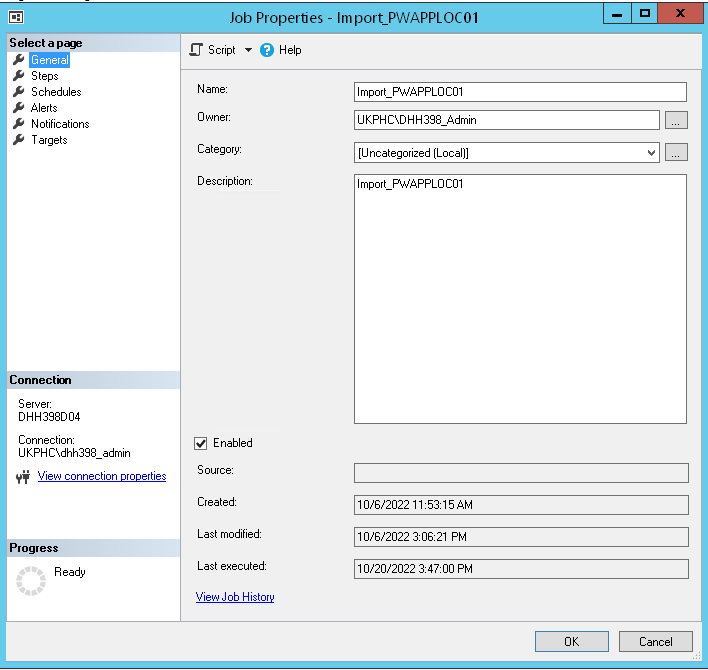
\includegraphics[width=0.7\textwidth, height=0.7\textheight,keepaspectratio]{immagini/M-schedulazione.png}
    \caption{Magazzino - Schedulazione aggiornamento database}
    \label{fig:M-Schedulazione}
\end{figure}
Per l’aggiornamento dei dati si è scritto il seguente codice:\\
    \texttt{delete from [dbo].[nome]\\
    DECLARE @SQLStr1 varchar(max)\\
    set @SQLStr1 =\\
    INSERT INTO [dbo].[nome] select *\\
    from OpenRowset('MSDASQL', select * FROM '\textit{nome}' )AS a\\
    EXECUTE(@SQLStr1);\\
    END}\\
\textit{Cioè prima si ripulisce il file e poi si importa nuovamente il tutto. L’eliminazione e la nuova importazione totale è più conveniente dell’aggiornamento dei singoli record in quanto si riduce il rischio di errore, si alleggerisce l’operazione non dovendo fare un continuo controllo tra i due file i quali potrebbero anche non essere ugualmente ordinati e ciò comporterebbe un ulteriore rallentamento.}\\
L’applicazione come da richiesta è stata sviluppata in un’unica schermata: oltre alla scannerizzazione e scrittura del barcode, nella parte alta si trovano le informazioni da visualizzare mentre nella seconda parte l’elenco delle locazioni specifiche di quell’articolo.\\
Nel database più record contengono lo stesso codice articolo e varia solo la locazione e relativa giacenza; quindi, sia per evitare di essere ripetitivi sia per fornire informazioni compatte a vista d’occhio in un’unica schermata, nella prima parte le informazioni vengono visualizzate una sola volta mediante questa formula nel suo contenitore generale:\\
\texttt{FirstN(Filter(Search([@PWAPPLOC01];TextInput1.Text;"IBLITM");\\
        Len(TextInput1.Text)=Len(TrimEnds(IBLITM)));1)
       }\\
\textit{Cerca nel database i record con il campo codice articolo (IBLITM) corrispondente a ciò che è scritto nella cella di input; filtra solo quelli che hanno lunghezza esattamente uguale alla lunghezza del codice inserito nella cella di input (calcolata con la funzione Trim per togliere gli spazi vuoti finali); filtra solo il primo record.}\\
Nella seconda parte per visualizzare l’elenco delle locazioni la formula è uguale ma senza il restringimento al primo record e quindi si filtra un elenco di record. Per la visualizzazione effettiva dei dati sono necessarie singole celle di testo impostate sulla specifica colonna; la \figurename \space \ref*{fig:M-Applicazione} mostra la schermata dell'applicazione
\begin{figure}[H]
    \centering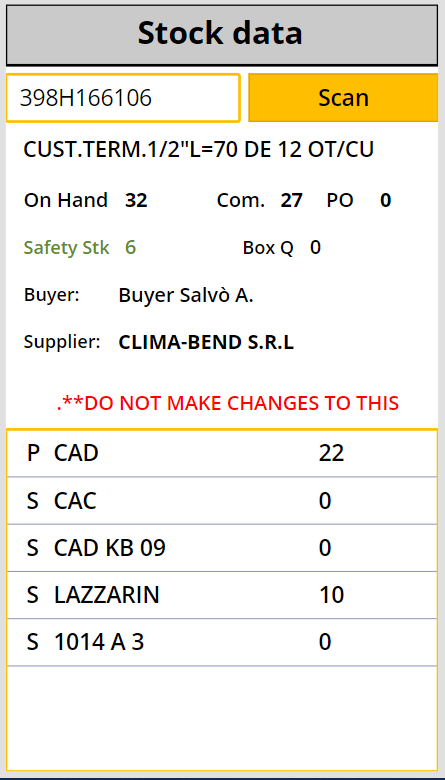
\includegraphics[width=0.4\textwidth, height=0.4\textheight,keepaspectratio]{immagini/M-applicazione.png}
    \caption{Magazzino - Unica schermata applicazione dati del magazzino}
    \label{fig:M-Applicazione}
\end{figure}